%% IEEE MCSoC 2026 submission.
%% Class + style follow the IEEE Conference Proceedings convention (IEEE Xplore).
%% Page limit: 8 pages including references (per supervisor). Two-column, 10pt, US letter.
%% Build: latexmk -pdf main.tex   (needs IEEEtran.cls, IEEEtran.bst — present in MiKTeX)

\documentclass[conference]{IEEEtran}
\IEEEoverridecommandlockouts

\usepackage{cite}
\usepackage{amsmath,amssymb,amsfonts}
\usepackage{algorithmic}
\usepackage{graphicx}
\usepackage{booktabs}
\usepackage{textcomp}
\usepackage{xcolor}
\usepackage[hidelinks]{hyperref}

\graphicspath{{figures/}}

\begin{document}

\title{A Spiking Trajectory Memory for Predicting Repetitive Motion from Event Cameras}

\author{\IEEEauthorblockN{Sagi Taizi}
\IEEEauthorblockA{\textit{Dept.\ of Mathematics and Computer Science} \\
\textit{The Open University of Israel}\\
Ra'anana, Israel \\
sagisagi229000@gmail.com}
\and
\IEEEauthorblockN{Elishai Ezra Tsur}
\IEEEauthorblockA{\textit{Neuro-Biomorphic Engineering Lab} \\
\textit{The Open University of Israel}\\
Ra'anana, Israel \\
elishai85@gmail.com}
}

\maketitle

\begin{abstract}
%% ~150--230 words, one paragraph, no citations, no custom macros.
%% State: problem, gap, what we do, how it is evaluated, headline result, why it matters.
% Placeholder. Event cameras report per-pixel brightness changes with microsecond latency,
% making them a natural sensor for anticipating fast, repetitive target motion. We present a
% spiking network that observes a target moving in a repeating path, builds a memory of that
% path online, predicts its position a short horizon ahead, and signals when the motion stops
% matching the learned pattern. The network is pretrained on trajectories rendered through a
% calibrated event-camera simulator and evaluated, with frozen weights, on real recordings of
% fan-driven, pendulum, hand-moved, and motor-driven motion. We report prediction error,
% lock-on time, and deviation-detection latency against classical periodic baselines. The
% contribution is a spiking formulation of trajectory anticipation as predictive inference,
% positioned as a component of a low-latency neuromorphic tracking pipeline.
\end{abstract}

\begin{IEEEkeywords}
event camera, spiking neural network, trajectory prediction, online learning,
novelty detection, neuromorphic vision
\end{IEEEkeywords}

\begin{figure*}[t]
\centering
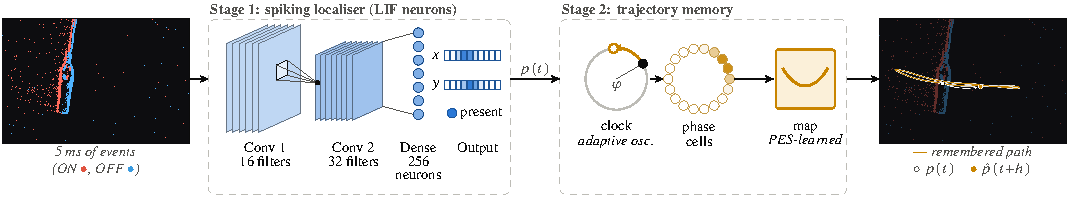
\includegraphics[width=\textwidth]{pipeline}
\caption{The proposed system. Stage~1: each 5~ms frame of accumulated ON and OFF events (left) passes through two convolutional LIF layers ($5\times5$ filters) and a dense layer of 256 LIF neurons, whose output gives the target's position $p(t)$ as place cells along $x$ and $y$ and a boolean indicating whether the target is visible. Stage~2: a clock implemented as an adaptive-frequency oscillator built from LIF neurons syncs with the motion, so its phase $\varphi$ tracks how far through each cycle the target is. A ring of phase cells then fires at the current detected phase, and a map, learned by a PES rule, holds the target's position at each phase. The prediction (right) $\hat{p}(t{+}h)$ is the map read at the next phase $\varphi{+}\omega h$, where $\omega$ is the clock's rate, and the remembered path is the map read at every phase over one full cycle.}
\label{fig:pipeline}
\end{figure*}

\section{Introduction}
Sight is by far the dominant sense humans use to perceive the world around them \cite{Gallego2022Event}. The retina, a thin sheet of tissue in the eye, converts raw light into nerve signals that we then interpret as visual images. However, a flash of light can evoke a neural response in the brain with a delay of 30--100 ms \cite{Berry1999Anticipation}, during which a moving target can cover a significant distance and should therefore be seen behind its actual position. As this contradicts our daily experience, it has been suggested that the brain acts as a `prediction machine', modelling what comes next and attending to what deviates \cite{Clark2013Whatever}. This is most striking for repetitive motion, where the eyes can lock on to a moving target within a few cycles and follow it with almost no lag \cite{Barnes1991The}.

The retina itself has a silicon counterpart \cite{Mahowald1991The}. Event cameras are low-power sensors that sample light based on the scene dynamics, and report per-pixel brightness changes as a stream of events with microsecond latency \cite{Gallego2022Event}. Spiking neural networks (SNNs) mimic the neurons behind it, computing via asynchronous discrete spikes which are sparse in time and allow for lower energy consumption and use with noisy inputs. Yet most pipelines built using them for tracking purposes react rather than anticipate---locating the target and extrapolating its position. A target that repeats its motion is exactly the case where prediction is possible, and event cameras and SNNs together are the parts from which such a biologically inspired prediction machine can be built. Such a system is useful in any application where a quick signal indicating that a target has deviated from its expected path is needed, for example in industrial inspection, robotics, and autonomous vehicles \cite{Sho2026A,Thoduka2021Using}. 

A target oscillating in a repetitive manner generates events in a periodic pattern. The task at hand is to learn this pattern from the event stream alone, predict the target's position a short horizon ahead, and signal when the motion stops matching. Real object movement, however, is never perfect--period and amplitude can drift and events can carry sensor noise, so the system must distinguish between these natural variations and actual deviation. For real-world scenarios, learning and detection must be performed online and without prior knowledge of the target's motion.

Separate parts of this problem have been previously addressed. Classical periodic filters like the Kalman filter \cite{Kalman1960A} predict repetitive motion well, but they assume a clean stream of accurate positions and are not spiking by nature. SNNs on event cameras have been used to predict trajectories, but primarily for one-shot motions and without a deviation signal (Section~\ref{sec:related}).

In this work, we propose a spiking system for online prediction built in two stages and tested on real-world cases using a real event camera. The first, a spiking localiser, estimates the target's position from short windows (5~ms) of accumulated events. Implemented with snnTorch \cite{Eshraghian2022Training}, it is trained with backpropagation through time (BPTT) using surrogate gradients \cite{Neftci2019Surrogate} on simulated clips and kept fixed. The second, a spiking memory built with the Neural Engineering Framework in Nengo \cite{Eliasmith2003Neural,Bekolay2014Nengo}, uses the localiser's output to learn the target's trajectory online. It relies on the fact that a repetitive motion with a defined cycle can be described by two things--where the target is at each point of the cycle--a map, and where in the cycle the target is now--a clock. The clock is an adaptive-frequency oscillator that locks on to the motion's rhythm \cite{Righetti2006Dynamic}, and the map is learned online on top of it. Once the map has settled, a copy of it is kept as the remembered path and updated only slowly from then on, and a deviation is flagged when the target moves too far from it.

The main contributions of this paper are as follows:
\begin{itemize}
\item A spiking trajectory memory built from a clock and a map that learns a repetitive path online without any pretraining, and predicts the target's position a short horizon ahead.
\item A deviation signal read from the same memory, which compares the target's position against a slowly updated copy of the learned path and raises an alarm within a fraction of a motion cycle and with no false positives.
\item An evaluation of the full pipeline on real event-camera motion of a swinging pendulum and other repetitive trajectories, with a localiser trained on simulated data only, against classical periodic baselines and manual annotations.
\end{itemize}
The rest of the paper is organised as follows--Section~\ref{sec:related} reviews related work, Section~\ref{sec:method} describes the method, and Section~\ref{sec:setup} the experimental setup. Section~\ref{sec:results} presents the results, which are discussed in Section~\ref{sec:discussion}, and Section~\ref{sec:conclusion} concludes the paper.

\section{Related Work}
\label{sec:related}
% Periodic-motion models: Harvey 1989 (structural time series, trigonometric seasonal
% component) -- phase and shape of a cycle held separately, the model behind the Kalman
% baseline, but with the period known in advance; our clock finds it. Pair with Gams et al.
% 2009 (adaptive oscillator + online-learned waveform, non-spiking, no deviation signal).
% Neither is in refs.bib yet; entries in BIBLIOGRAPHY.md.

\section{Method}
\label{sec:method}

Our proposed system is a spiking pipeline built from two stages of SNNs as seen in Fig.~\ref{fig:pipeline}. Events from the camera are accumulated into short 5ms frames from which a spiking localiser estimates the target's position in the scene. Given this constant stream of positions, the trajectory memory SNN learns the target's path, predicts where the target will be a short time ahead, and flags when motion departs from the estimated path. The localiser is trained once on simulated data only and kept fixed, while the memory is not trained in advance and learns online. Section~\ref{sec:problem} defines the task while the event input, localiser, memory and the deviation score are described in Sections~\ref{sec:input}--\ref{sec:deviation}.

\subsection{Problem Setup}
\label{sec:problem}
A static event camera observes a single target moving along a repetitive path. Let $p(t)$ denote the target's position in the image at time $t$, in pixels. The motion is repetitive in the sense that $p(t+T) \approx p(t)$ for a period $T$ of about one to a few seconds, which is not known in advance. The approximation is deliberate: real motion drifts, its amplitude decays or grows, and its period varies slightly from cycle to cycle, and these natural variations are part of the normal motion.

From the event stream alone, and processing it once in the order it arrives, the system must produce two outputs at every time step: a prediction $\hat{p}(t+h)$ of the target's position a fixed horizon $h$ ahead, and a scalar deviation score $s(t)$. We report horizons of 25 to 200~ms, with $h = 100$~ms as the main one. A deviation is a change after which the motion no longer follows the learned path, such as a push that changes the amplitude or the direction of the swing, or a change in speed; the score should stay low under natural variations and rise quickly after a deviation. Neither the path, nor its period, nor the time of a deviation is given to the system. Re-learning a new path after a deviation is left for future work.

\subsection{Event Input}
\label{sec:input}
The events are recorded with a DVXplorer event camera ($640\times480$ pixels) held still. Each event $e=(x, y, t, q)$ reports a brightness change at pixel $(x, y)$ at time $t$, with polarity $q$ marking an increase (ON) or a decrease (OFF). The stream is cut into consecutive windows of 5~ms, and each window is accumulated into a frame of two channels, counting the ON and the OFF events at every pixel. The frames are then reduced $8\times$ by summing $8\times8$ blocks, giving a $2\times60\times80$ input for every 5~ms step. The window length sets how often the system produces an output and how long it waits for its input, and is the main latency parameter of the pipeline.

As a classical alternative to the spiking localiser, used as input by the baselines and in the ablations, the target's position is also estimated directly from the events: the events of a window are counted in cells of $16\times16$ pixels, the cells holding at least 30\% of the fullest one are kept, and the position is the mean of their events. This keeps the estimate on the dense target rather than on noise spread over the sensor or on a thin string above a hanging target, and we refer to it as the classical centroid.

\subsection{Localiser}
\label{sec:localiser}
The localiser is a convolutional spiking network that runs once per frame and carries the state of its neurons from one frame to the next (Fig.~\ref{fig:pipeline}, Stage~1). Two convolutional layers of $5\times5$ filters with a stride of 2 map the input to 16 feature maps of $30\times40$ and then to 32 feature maps of $15\times20$, and a fully connected layer of 256 neurons follows. All three layers are made of leaky integrate-and-fire (LIF) neurons, whose membrane potential integrates the input, leaks with a time constant of 10--20~ms, and emits a spike when it crosses a threshold. The leak gives the network a short memory of the last few frames, so a frame with few events is still read in the light of the frames before it.

The spikes of the last layer are smoothed with a 15~ms filter and read out linearly into 65 values: 32 place cells for $x$, 32 for $y$, and a single unit that indicates whether the target is visible at all. Each place cell stands for one position along its axis, and the position is read as the centre of mass of the cells' activity along each axis. When the target is reported as not visible, the step is passed on to the memory as unseen and is skipped.

The network is implemented in snnTorch \cite{Eshraghian2022Training} and trained with backpropagation through time using surrogate gradients \cite{Neftci2019Surrogate}, over chunks of 0.25~s with the state carried between them. The loss compares the place cells of each axis with a Gaussian bump centred on the true position, adds a binary term for visibility, and keeps the dense layer firing at about 10\% of steps. Training uses simulated recordings only (Section~\ref{sec:setup}), 300 clips of a target moving along varied paths, and adds to them the imperfections of the real camera that the simulator does not produce: stuck pixels, a background of noise events, mirror flips and a quarter turn, a random brightness scale, an exchange of the ON and OFF channels, and short stretches in which the target is removed. The network is trained for 20 epochs, and for the pendulum it is then fine-tuned for 10 more on simulated pendulum recordings. The weights are fixed before any real recording is used.

\subsection{Trajectory-Memory Network}
\label{sec:memory}
The memory receives the target's position every 5~ms and learns, online, where the target is at each point of its cycle (Fig.~\ref{fig:pipeline}, Stage~2). It consists of a clock that follows the phase of the motion, a ring of phase cells that represents that phase, and a map from the phase cells to position.

\emph{Clock.} The motion is first reduced to a single signal $F(t)$: the position projected on the main axis of the motion, found online from a running estimate of the positions' covariance, and scaled to a unit amplitude. The clock is an adaptive-frequency oscillator \cite{Righetti2006Dynamic}, whose state $(x_c, y_c)$ turns around a limit cycle at a rate $\omega$ while $F$ pulls on its phase $\varphi$ and, more slowly, on its rate:
\begin{align}
\dot{x}_c &= \gamma(1-r^2)\,x_c - \omega\,(1-\kappa F y_c)\,y_c, \nonumber\\
\dot{y}_c &= \gamma(1-r^2)\,y_c + \omega\,(1-\kappa F y_c)\,x_c, \label{eq:clock}\\
\dot{\omega} &= -\eta_\omega\,\omega F y_c, \nonumber
\end{align}
with $r^2 = x_c^2 + y_c^2$, $\varphi = \mathrm{atan2}(y_c, x_c)$, $\gamma = 2$, $\kappa = 0.3$ and $\eta_\omega = 0.6$. After a few cycles the rate matches the period of the motion and the phase keeps a fixed relation to it, so $\varphi$ tells how far through its cycle the target is. The clock's state, together with $\omega$ and $F$, is represented by a population of 1,500 LIF neurons, and the recurrent connections that make the population follow \eqref{eq:clock} are found with the Neural Engineering Framework \cite{Eliasmith2003Neural} in Nengo \cite{Bekolay2014Nengo}. The rate itself is updated outside the population and fed back into it, since holding it as a neural integrator made it drift. Six clocks, started at periods between 0.8 and 7~s, run side by side, and the one whose period agrees with the period measured from the crossings of $F$ through zero is used.

\emph{Phase cells.} The phase is passed to a ring of 400 LIF neurons, each tuned to one direction on the unit circle, as the unit vector $(\cos\varphi, \sin\varphi)$. At any moment the neurons tuned near $\varphi$ fire, forming a bump of activity $a(t)$ that travels around the ring as the clock turns.

\emph{Map.} The map is a set of connections $W$ from the phase cells to the target's position, which starts empty in every recording and is learned by an error-driven rule of the PES family \cite{MacNeil2011Fine}:
\begin{equation}
\Delta W = \eta\,\frac{\big(p(t) - W a(t)\big)\,a(t)^{\top}}{\lVert a(t)\rVert^{2}},
\end{equation}
where the learning rate $\eta$ decays from 0.3 to 0.02 over the first seconds of motion. Each update moves the position stored at the active phase towards the observed one, so after a few cycles $W$ holds the target's path, one position per phase. A slow correction of the output's centre and scale follows gradual changes of the path, such as the decaying amplitude of a pendulum, and once a clock is chosen, a position far from where the map expects the target is treated as unseen, which protects the map from a momentary error of the localiser.

\emph{Prediction.} To predict $h$ ahead, the phase is advanced by $\omega h$ and the map is read through the ring's tuning at the advanced phase, $\bar{a}(\varphi + \omega h)$:
\begin{equation}
\hat{p}(t+h) = W\,\bar{a}(\varphi + \omega h) + e^{-h/\tau_r}\,\rho(t),
\end{equation}
where $\rho(t)$ is the recent error of the map, smoothed over 20~ms, which lets the prediction follow a target that is momentarily off its path, and $\tau_r = 2$~s. The neurons of the clock and the ring use Nengo's LIF model (membrane time constant 20~ms, refractory period 2~ms) and are simulated in PyTorch in steps of 1~ms, five per frame.

\subsection{Deviation Score}
\label{sec:deviation}
If the deviation were measured against the map itself, the map would learn the new motion within a few cycles and the deviation would disappear from the score. The score is therefore measured against a second copy of the map, $W_s$, taken once the memory has settled: when the chosen clock has run for at least three cycles, its period agrees with the one measured from $F$, and the map's error has stopped decreasing. From then on $W_s$ follows the working map only slowly, with a time constant that grows to 30~s, so it keeps the path as it was learned. The deviation score is the distance between the observed position and the position that $W_s$ holds for the current phase,
\begin{equation}
s(t) = \big\lVert p(t) - W_s\,a(t) \big\rVert,
\end{equation}
smoothed over 0.2~s.

An alarm is raised when $s(t)$ stays above a threshold for three consecutive steps (15~ms). The threshold is set from the score itself and needs no labels: over a sliding window of 2~s it is the median of the score plus $k$ times its spread (the scaled median absolute deviation), and it only ever decreases, taking the lowest value reached so far. It therefore tightens while the memory settles and cannot be raised by the deviation it is meant to catch. The constant $k$ is chosen once on the development recordings for each input (Section~\ref{sec:protocol}).

\section{Experimental Setup}
\label{sec:setup}

\subsection{Event-Camera Simulator}
% v2e configured with the DVXplorer intrinsics, lens distortion, contrast threshold, noise.
% Trajectory families: circle, ellipse, figure-eight, Lissajous; scripted deviations.
% Start: v2e's EventEmulator (Hu, Liu, Delbruck 2021) fed a 650 fps render of a target on
% an analytic path, DVXplorer 640x480 through the calibrated lens model; ground truth is the
% target's APPARENT (distorted) position, the same thing hand-labels record. Matched to the
% real fan clip on five statistics (real vs sim): target rate 82.0k vs 84.5k ev/s, ON
% fraction 0.509 vs 0.504, blob footprint 18.2 vs 18.4 px, trail behind the target 19.6 vs
% 17.1 px, noise floor 0.105 vs 0.088 ev/px/s (median 32 px tile). Photoreceptor filter off:
% v2e scales its time constant by intensity and left a 60--90 ms event trail behind fast
% targets that the real camera does not show. Per-clip domain randomisation: thresholds
% 0.15--0.30, sigma 0.01--0.06, shot noise 0.03--0.5 Hz/px, contrast, radius 8--30 px, aspect
% 1--4 (disc to brush), a string to a pivot (half the clips), body texture, an optional
% 60--200 Hz lag (half); paths from five families (circle, ellipse, straight sweep,
% figure-8, Lissajous), T 0.8--4 s, half with one scripted deviation in the middle third,
% 30% exact and the rest with small smooth imperfections. Corpus summary table: see
% materials/02-methods/simulation-with-v2e.md (added once the 100 clips are generated).

\subsection{Real Recordings}
% Four regimes: ceiling-fan (circular), string pendulum, hand-moved, motor-driven on a blank
% wall (exact encoder ground truth via calibration). Single high-contrast target; daylight.
% NOTE the line above is stale: the encoder ground truth was abandoned (PAPER_PROGRESS.md);
% ALL ground truth is hand-labels + linear interpolation, every setup, 4a included.
% Start: 54 clips recorded 2026-09-10 (RECORDING_LOG.md), 14 with a deviation; evaluated on
% 6 development + 11 held-out (PLAN.md table). Per regime, give period / amplitude / rate:
% fan brush on a string, a rigid 74x46 px ellipse, T = 1.19 s, 165k ev/s; pendulum brush,
% T = 1.18--1.27 s, 135--430 px swings, 0.6--1.5M ev/s, with a visible string; hand-moved
% wall target: straight sweeps of ~160 px at T = 1.8 s and 1.0 s, 0.3--1M ev/s, marginal
% SNR; motor-swept scene (4a): the whole scene moves, T = 1--4 s, reported as a separate
% condition. Labelling: one mark per 0.1 s (pendulum), 0.15 s (fan), 0.25 s (wall target);
% the fan labels sit 4.5 px (median) from a fitted ellipse. Convention caveat to state: the
% marked point is the brush centre, which sits 27--43 px below the event centroid on the
% pendulum -- how that is handled belongs in Metrics. Fig. 2: one accumulated frame per
% setup, from scripts/replay_gt.py --save.

\subsection{Baselines}
% Periodic Kalman filter; harmonic / Fourier fit; rhythmic dynamic movement primitive.
% Start (two are implemented, trajmem/baseline.py; the DMP only if it gets built):
% (1) Kalman filter with a harmonic state per coordinate, [mean, (c_k, d_k) k = 1, 2],
% each pair rotating at k*omega per step; q = 1e-6, r = 1e-4 (normalised units); the
% prediction is the same rotation carried to t+h; surprise = normalised innovation, smoothed
% with tau = 100 ms. (2) Sliding least-squares harmonic fit (2 harmonics, last 3 periods),
% evaluated at t+h; surprise = distance of the new observation from the previous fit,
% relative to that fit's residual spread. Both estimate T from a 5 s warm-up by residual
% search and keep it (stated in the protocol below). Development-set numbers at 100 ms (runs/results/development_*.csv,
% Kalman / harmonic, px median): fan 8.0 / 7.3; pendulum 26--48 (label offset dominates);
% wall target 19--56; pooled 24.2 / 32.6. Simulated clips with exact truth: ~3 px. Breaks:
% wide_break AUC 0.86 / 0.67, loop_break_01 0.75 / 0.81. Frame these as the accuracy bar the
% spiking version must meet on clean motion, per the claim in the Introduction.

\subsection{Evaluation Protocol}
\label{sec:protocol}
The real recordings are never used for training or fine-tuning and are divided in advance into development recordings, which were used freely while building the system and to choose the alarm constant, and held-out recordings, which were labelled last and scored once, after every setting had been fixed. The alarm constant is the smallest value that detects every deviation in the development recordings without a false alarm, and it is applied unchanged to the held-out ones.

Every method, spiking or classical, receives the same stream of positions, one every 5~ms, from the same localiser, and none is given the period of the motion. The classical baselines estimate the period from the first 5~s of each recording and keep it, while the memory finds it through its clock. Prediction errors are measured from the sixth second of a recording, once every method has had time to learn the motion, and up to the start of any deviation.

\subsection{Metrics}
% Prediction error at the horizon; lock-on time; deviation-detection ROC and median latency.
% Start (definitions as implemented in trajmem/metrics.py, after materials/02-methods/
% metrics.md): error = Euclidean distance in px between p^(t+h) and truth at t+h, over the
% scoring window set in the protocol above, reported as median and IQR per clip and pooled
% as the median of per-clip medians; lock-on = first time after which the error stays under
% a tolerance for the rest of the clip, in seconds and in cycles, tolerance stated per
% regime; deviation: positives are steps at or after the break, AUC is Mann--Whitney over
% the score, a flag is the alarm of the Deviation Score section (refer, don't redefine),
% latency is the first flag after the break, false alarms are flags per minute on
% negatives. Decide and state here how the pendulum's
% constant label offset is handled: subtract the per-clip median offset, or score prediction
% against the frontend's own track and report localisation against labels separately.

\section{Results}
\label{sec:results}
% DRAFT (2026-09-25, overnight). Numbers from scripts/paper_results.py + paper_figures.py
% (runs/paper/, tables in runs/paper/tables.tex). Held-out = the three pendulum clips, each
% scored once; the fan, wall-target and 4a held-out clips are not labelled yet. Pendulum
% positions are scored against the labels as they stand; fan and wall target with each
% clip's constant label offset removed (Section~\ref{sec:setup}).

\subsection{Localiser}
\label{sec:res-localiser}
On the pendulum, the spiking localiser places the target far closer to the labelled point than the classical centroid does (Fig.~\ref{fig:localiser}). Over the six pendulum recordings, its median distance from the label is 14~px (90th percentile 28~px), against 65~px (125~px) for the centroid. The gap is widest on the held-out recordings, 12 against 98~px, where the centroid settles on a different part of the target than the one marked. Most of the centroid's error is a constant offset: removing it per recording leaves 8--40~px, against 8--13~px for the spiking localiser. On the fan and the wall target, which the simulator resembles less closely, the spiking localiser brings no gain (fan 10~px against the centroid's 5~px; wall target 17--23~px for both), and the classical centroid remains their input in what follows.

\begin{figure}[t]
\centering
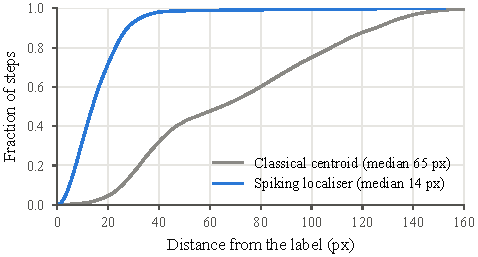
\includegraphics[width=\columnwidth]{results_localiser}
\caption{Localisation error on the six pendulum recordings (development and held-out), against the hand labels as they stand. The spiking localiser was trained on simulated data only.}
\label{fig:localiser}
\end{figure}

\subsection{Prediction and Path Memory}
\label{sec:res-prediction}
Table~\ref{tab:pendulum} and Fig.~\ref{fig:horizon} give the prediction error of the full spiking pipeline on the pendulum. At short horizons the spiking memory is close to the classical periodic baselines: on the held-out recordings its median error is 14.2~px at 50~ms, against 12.2~px for the periodic Kalman filter and 10.5~px for the harmonic fit. As the horizon grows it falls behind them, reaching 18.0~px at 100~ms and 24.4~px at 200~ms, while both baselines stay near 11--14~px. On the development recordings the three methods are within 4~px of each other up to 100~ms. All three periodic methods do far better than a constant-velocity extrapolator beyond 50~ms, whose error grows with the horizon to 60~px at 200~ms on the held-out recordings.

The remembered path matches the labelled one to a median of 18~px on the held-out recordings (Kalman 14~px, harmonic fit 12~px), and the clock settles within 4\% of the true period on every pendulum recording, always slightly short. The baselines reach their steady error at the end of their five-second warm-up; the memory, which has no warm-up, reaches it about a second later, once its clock has locked and its map has filled, within five to six swings. On the fan and the wall target (Table~\ref{tab:other}), with the classical centroid as input, the ranking is the same at short horizons (15.3~px at 100~ms against 12.3~px for the Kalman filter); the harmonic fit is the least accurate predictor there but recalls the path best.
% NOTE for Sagi: this is weaker than the introduction's "on par" -- behind at 200 ms on the
% held-out pendulum. Revisit the claim in Section I or name the horizon it holds at.

\begin{table}[t]
\caption{Pendulum, full spiking pipeline, against the labels as they stand}
\label{tab:pendulum}
\centering
\footnotesize
\setlength{\tabcolsep}{2.3pt}
\begin{tabular}{lrrrrrrr}
\toprule
 & \multicolumn{3}{c}{Error at $h$ (px)} & Path & & Lat. & False \\
\cmidrule(lr){2-4}
Memory & 50\,ms & 100\,ms & 200\,ms & (px) & AUC & (s) & al./min \\
\midrule
\multicolumn{8}{l}{\emph{Held-out (3 recordings, 1 with a deviation)}} \\
\textbf{Spiking clock-and-map} & 14.2 & 18.0 & 24.4 & 18.0 & 0.98 & 0.07 & 0.0 \\
Clock-and-map, arith. & 13.8 & 18.3 & 25.9 & 16.8 & 0.99 & 0.26 & 0.0 \\
Periodic Kalman & 12.2 & 13.7 & 11.2 & 14.1 & 1.00 & 0.67 & 14.4 \\
Harmonic fit & 10.5 & 10.9 & 11.3 & 11.5 & 0.63 & -- & 1.4 \\
Constant velocity & 19.5 & 30.5 & 60.4 & -- & 0.70 & -- & 0.0 \\
\midrule
\multicolumn{8}{l}{\emph{Development (3 recordings, 1 with a deviation)}} \\
\textbf{Spiking clock-and-map} & 19.6 & 22.6 & 30.4 & 21.7 & 0.99 & 0.32 & 0.0 \\
Clock-and-map, arith. & 18.1 & 19.6 & 22.8 & 17.5 & 1.00 & 0.29 & 0.0 \\
Periodic Kalman & 21.7 & 21.3 & 20.7 & 20.1 & 0.99 & 0.16 & 1.0 \\
Harmonic fit & 19.1 & 19.0 & 18.9 & 17.4 & 0.70 & -- & 0.0 \\
Constant velocity & 28.7 & 45.8 & 102.9 & -- & 0.67 & -- & 0.0 \\
\bottomrule
\end{tabular}
\\[2pt]
{\scriptsize Errors and path: medians over recordings. AUC and latency: the recording with a deviation. False alarms: mean over recordings. A latency is left out where the detector does not separate the deviation (AUC $<$ 0.75).}
\end{table}

\begin{table}[t]
\caption{Fan and wall target (development), classical centroid input, constant label offset removed}
\label{tab:other}
\centering
\footnotesize
\setlength{\tabcolsep}{2.3pt}
\begin{tabular}{lrrrrrrr}
\toprule
 & \multicolumn{3}{c}{Error at $h$ (px)} & Path & & Lat. & False \\
\cmidrule(lr){2-4}
Memory & 50\,ms & 100\,ms & 200\,ms & (px) & AUC & (s) & al./min \\
\midrule
\textbf{Spiking clock-and-map} & 11.1 & 15.3 & 22.1 & 16.6 & 0.97 & 0.33 & 0.0 \\
Clock-and-map, arith. & 11.6 & 13.4 & 19.1 & 15.2 & 0.99 & 0.16 & 8.0 \\
Periodic Kalman & 10.0 & 12.3 & 16.0 & 16.7 & 0.76 & 0.37 & 44.6 \\
Harmonic fit & 23.5 & 24.7 & 26.1 & 8.7 & 0.74 & -- & 0.0 \\
Constant velocity & 12.0 & 17.9 & 47.3 & -- & 0.33 & -- & 0.0 \\
\bottomrule
\end{tabular}
\\[2pt]
{\scriptsize Three recordings; one contains a deviation.}
\end{table}

\begin{figure*}[t]
\centering
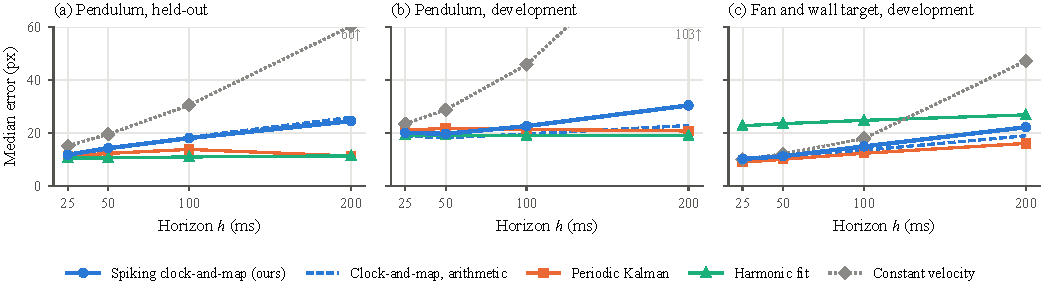
\includegraphics[width=\textwidth]{results_horizon}
\caption{Median prediction error against the horizon. (a,~b)~Pendulum through the full spiking pipeline, against the labels as they stand. (c)~Fan and wall target through the classical centroid, constant label offset removed. Values off the axis are printed at its top.}
\label{fig:horizon}
\end{figure*}

\subsection{Deviation Detection}
\label{sec:res-deviation}
The deviation signal is where the spiking memory stands out (Table~\ref{tab:pendulum}, Fig.~\ref{fig:break}). On the held-out pendulum deviation it raises its alarm 0.07~s after the deviation begins, with an AUC of 0.98 and no false alarm on any of the three held-out recordings. The periodic Kalman filter separates the deviation as well (AUC 1.00) but flags it only after 0.67~s, and raises 14 false alarms per minute on steady motion, 38 on one recording. The harmonic fit barely separates the deviation (AUC 0.63). The same holds on the development recordings: the spiking memory detects both deviations (pendulum and wall target) without a single false alarm, while the Kalman filter raises 45 false alarms per minute on the fan and wall-target recordings. The alarm threshold was chosen on the development recordings and applied unchanged to the held-out ones; with a single deviation per group, these latencies are indicative rather than statistical.

\begin{figure}[t]
\centering
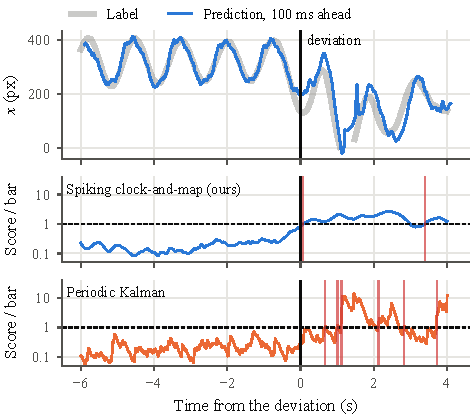
\includegraphics[width=\columnwidth]{results_break}
\caption{A held-out pendulum recording with a deviation, full spiking pipeline. Top: the target's horizontal position and the 100~ms prediction. Middle and bottom: each method's deviation score over its own alarm bar (dashed line at 1); red lines mark alarm onsets.}
\label{fig:break}
\end{figure}

\subsection{Ablations}
\label{sec:res-ablations}
\emph{Learned memories.} The two memories that learn the cycle as network dynamics, a recurrent network of fast and slow LIF layers trained on simulated tracks and a spiking Legendre Memory Unit that records a window of the past, do not hold the cycle (Fig.~\ref{fig:paths}). On the development pendulum recordings their remembered paths are 95 and 64~px from the labelled one, with periods 1.89 and 1.26 times the true one, and their 100~ms errors are 32 and 45~px against 23~px for the clock-and-map memory.

\emph{Spiking against arithmetic.} The clock-and-map memory written as plain arithmetic predicts within 0.5~px of the spiking one on the held-out pendulum up to 100~ms and detects the deviation equally well (AUC 0.99 against 0.98). The spiking version costs accuracy only at the longest horizon on the development recordings (30.4 against 22.8~px at 200~ms).

\emph{Input.} With the classical centroid in place of the spiking localiser, the spiking memory's 100~ms error against the pendulum labels rises from 18--32~px to 27--49~px on the development recordings and from 11--22~px to 76--130~px on the held-out ones, so on this setup the localiser sets the accuracy the whole pipeline can reach.

\begin{figure*}[t]
\centering
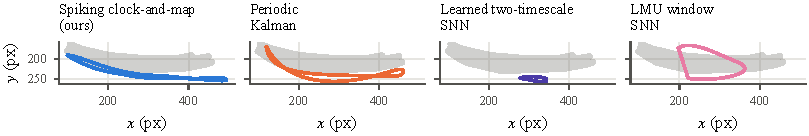
\includegraphics[width=\textwidth]{results_paths}
\caption{The remembered cycle of each memory just before the deviation in a development pendulum recording, over the labelled path of the preceding 6~s (grey), all through the spiking localiser. Only the clock-and-map memory and the Kalman filter hold the swing.}
\label{fig:paths}
\end{figure*}

\section{Discussion}
\label{sec:discussion}
% Where the spiking version wins / costs accuracy; event-native and latency arguments.
% Neuromorphic-hardware energy/latency: cited, not measured (no Loihi/Lava access).
% Limitations. Future work: online re-learning of a new pattern; attention across objects.

\section{Conclusion}
\label{sec:conclusion}
% One paragraph.

\section*{Acknowledgment}
% Supervision, lab, funding.
% Start: one or two sentences -- Dr. Elishai Ezra Tsur's supervision; the Neuro-Biomorphic
% Engineering Lab (Open University of Israel) for the DVXplorer and the pan-tilt rig; any
% funding line the lab requires. No reviewers-thanks in the submitted version (double-blind
% check: confirm with the CFP whether author names must be removed at submission).

\label{sec:impl}
% If space allows, a short implementation-notes paragraph or move framework details here.

\bibliographystyle{IEEEtran}
\bibliography{refs}

\end{document}
